\documentclass{article}
\usepackage[margin=1in]{geometry}
\usepackage{tikz}
\usetikzlibrary{arrows.meta, shapes.geometric, positioning}
\usepackage{amsmath}
\begin{document}

\title{Software Architecture Layout}
\author{}
\date{}
\maketitle

\section{Software Plan}
Using camera + IR/color sensor combination.

\subsection*{Infrastructure}
\begin{itemize}
\item Use a state machine to track the current program stage.
\item Start in \texttt{LINE\_READING}, which fuses IR array signals and the camera frame to compute motion commands.
\item If only one line is detected: calculate the line length $L_k$.
\item Else: calculate the intersection first, then compute the line length $L_k$.
\item Use $L_k$ and the current speed to obtain the fuzzy mode and PID parameters.
\end{itemize}

\section{State Machine Flowchart}
\begin{center}
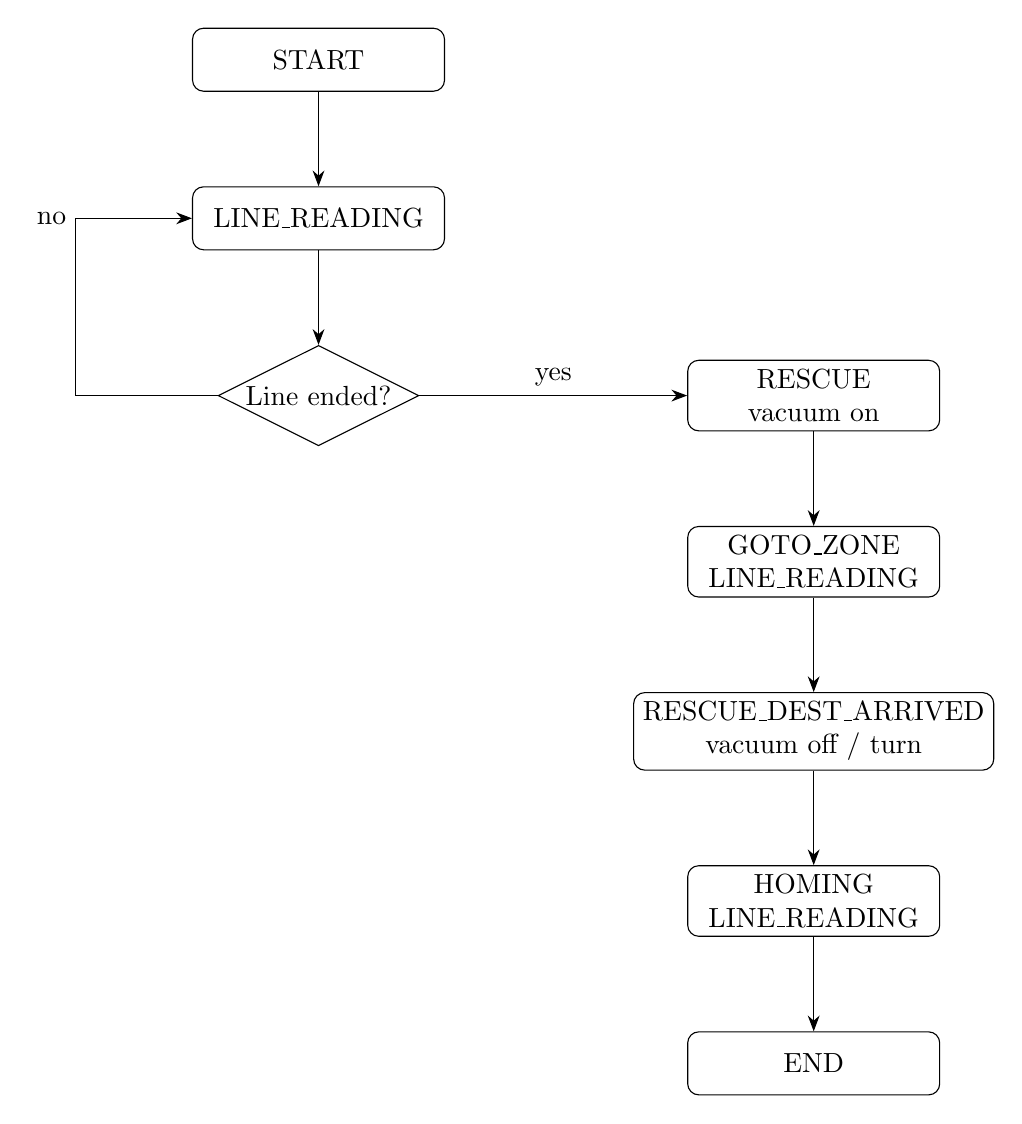
\begin{tikzpicture}[
    node distance=12mm and 18mm,
    state/.style={rectangle, rounded corners, draw, align=center, minimum width=32mm, minimum height=8mm},
    decision/.style={diamond, draw, align=center, aspect=2, inner sep=1pt},
    arrow/.style={-{Stealth[length=2mm]}}
]
    \node[state] (start) {START};
    \node[state, below=of start] (line) {LINE\_READING};
    \node[decision, below=of line] (ended) {Line ended?};

    \node[state, right=of ended, xshift=16mm] (rescue) {RESCUE\\vacuum on};
    \node[state, below=of rescue] (goto) {GOTO\_ZONE\\LINE\_READING};
    \node[state, below=of goto] (arrive) {RESCUE\_DEST\_ARRIVED\\vacuum off / turn};
    \node[state, below=of arrive] (home) {HOMING\\LINE\_READING};
    \node[state, below=of home] (end) {END};

    \draw[arrow] (start) -- (line);
    \draw[arrow] (line) -- (ended);
    \draw[arrow] (ended.east) -- node[above]{yes} (rescue.west);
    \draw[arrow] (ended.west) -- ++(-18mm,0) |- node[left]{no} (line.west);

    \draw[arrow] (rescue) -- (goto);
    \draw[arrow] (goto) -- (arrive);
    \draw[arrow] (arrive) -- (home);
    \draw[arrow] (home) -- (end);
\end{tikzpicture}
\end{center}

\section{Node-by-Node Behavior}
\begin{itemize}
\item \texttt{START}: initialize sensors, camera, communication, and motor driver; set initial mode and variables.
\item \texttt{LINE\_READING}: run the closed-loop line follower by fusing IR error and camera line-length information to generate left/right motor commands.
\item \texttt{Line ended?}: decision node; if the main line is no longer detected, transition to rescue sequence, otherwise continue \texttt{LINE\_READING}.
\item \texttt{RESCUE}: stop or slow as required, activate the vacuum mechanism, and secure the Lego figure.
\item \texttt{GOTO\_ZONE / LINE\_READING}: navigate to the drop-off zone using the same line-reading controller (IR + camera + fuzzy/PID scheduling).
\item \texttt{RESCUE\_DEST\_ARRIVED}: perform destination action (optional turn based on zone orientation), then deactivate vacuum to release the Lego figure.
\item \texttt{HOMING / LINE\_READING}: follow the return path home using line reading again, with mission-complete constraints if needed (e.g., reduced speed).
\item \texttt{END}: stop motors, place actuators in safe state, and terminate or idle.
\end{itemize}

\section{LINE\_READING Loop (Camera + IR Fusion)}
\begin{verbatim}
loop:
  ir = read_IR_array()
  err = line_position(ir) - center
  pid_u = PID(err, Kp, Ki, Kd)

  frame = camera_capture()
  lines = detect_line_vectors(frame)
  Lk = compute_primary_line_length_or_intersection(lines)

  X1 = speed_percent(current_speed)
  X2 = lookahead_percent(Lk)

  mode = fuzzy_or_table(X1, X2)
  baseSpeed, (Kp, Ki, Kd) = mode_parameters(mode)

  left  = clamp(baseSpeed - pid_u)
  right = clamp(baseSpeed + pid_u)
  set_motors(left, right)
\end{verbatim}

\section{Notes}
\begin{itemize}
\item $X_1$ is the current speed command normalized to 0--100.
\item $X_2$ is the visible line length percentage computed from the camera ROI.
\item The state machine transitions to \texttt{RESCUE} when the line ends, then to \texttt{GOTO\_ZONE}, \texttt{RESCUE\_DEST\_ARRIVED}, and \texttt{HOMING}.
\end{itemize}

\end{document}
